%
% interpolacao.tex (LateX)
% 
% Objetivo: Capítulo sobre a etapa de interpolação do relatório de qualificação de doutorado.
% 
% Versão 1.0
% 
% Site: http://www.dirackslounge.online
% 
% Programador: Rodolfo A. C. Neves (Dirack) 17/10/2019
% 
% Email: rodolfo_profissional@hotmail.com
% 
% Licença: GPL-3.0 <https://www.gnu.org/licenses/gpl-3.0.txt>.

\chapter{INTERPOLAÇÃO COM FILTROS ADAPTATIVOS DE PREDIÇÃO DE ERRO}

A etapa de intepolação permite aumentar a amostragem dos dados modelados, de 0.025Km no afastamento, para 0.0125Km.
Isto é importante para montar as seções ERC, com os traços cujas coordenadas $m$ e $h$ estão o mais próximo possível
das coordenadas $m$, $h$ da curva ERC calculada.

Obviamente, poderíamos ter realizado a etapa de modelagem com uma discretização maior, porém o intuito é mostrar como
a intepolação com filtros de erro adaptativos pode regularizar a amostragem dos dados, possibilitando a busca pelos
traços que estão sobre as trajetórias ERC com a maior precisão possível.

Antes da interpolação, os dados sísmicos nas coordenadas $m$ e $h$ são separados em seções de afastamento constante.
A interpolação com os filtros adaptativos de predição de erro (FPE) é realizada para cada seção, aumentando assim a
sua discretização (de 0.025Km para 0.0125Km). Após esta etapa, calculamos as trajetórias ERC para cada $m0$, e determinamos
as coordenada $m$, $h$ dos pontos sobre estas trajetórias que intersectam as seções de afastamento constante. Estes pontos
$m$, $h$ serão as coordendas dos traços que pertencem à trajetória ERC, por definição.

Com o conhecimento das coordenadas $m$, $h$ dos traços sobre a ERC, determinados anteriormente, buscamos nas seções interpoladas
os traços sísmicos com as coordenadas $m$ e $h$ mais próximas das trajetórias ERC calculadas, e montamos as seções ERC. 
Cada PMC $m0$ possuirá uma seção ERC e parâmetros $R_N$, $R_{NIP}$ e $\beta_0$; e cada par $m0$, $t0$ terá uma curva de tempo
de trânsito ERC correspondente. O empilhamento ERC é realizado sobre as curvas de tempo de trânsito ERC,, somando as amplitudes
das amostras sobre a curva e atribuindo esta soma aos pares $m0$, $t0$ na seção empilhada ERC.

A Figura \ref{fig:6.1}-\ref{fig:6.2} apresentam as seções ERC organizadas pela coordenada do afastamento $h$. A Figura
\ref{fig:6.1} é a seção ERC para o $m0=5Km$ e as Figuras \ref{fig:6.2}-\ref{fig:6.3} para o $m0=4Km$. O ajuste feito com
a equação de tempo de trânsito ERC (pontos em amarelo) depende também da escolha do tempo $t0$. Na Figura \ref{fig:6.3}, 
o $t0=1.1s$ utilizado não é apropriado, não produzindo o melhor ajuste. Portanto, o empilhamento sobre as curvas que possuam
os melhores ajustes com os dados modelados tendem a produzir somas construtivas, enquanto o empilhamento sobre curvas de
pior ajuste, tendem a produzir somas destrutivas.

\begin{figure}
\caption{Seção CRE para o PMC $m0=5Km$ e $t0=1.1s$.
Pontos em amarelo representa a curva de tempo de trânsito ERC sobre a qual
será realizado o empilhamento ERC.
O eixo horizontal é a coordenada do afastamento $h$ e o eixo vertical o tempo
$t$.}
\begin{center}
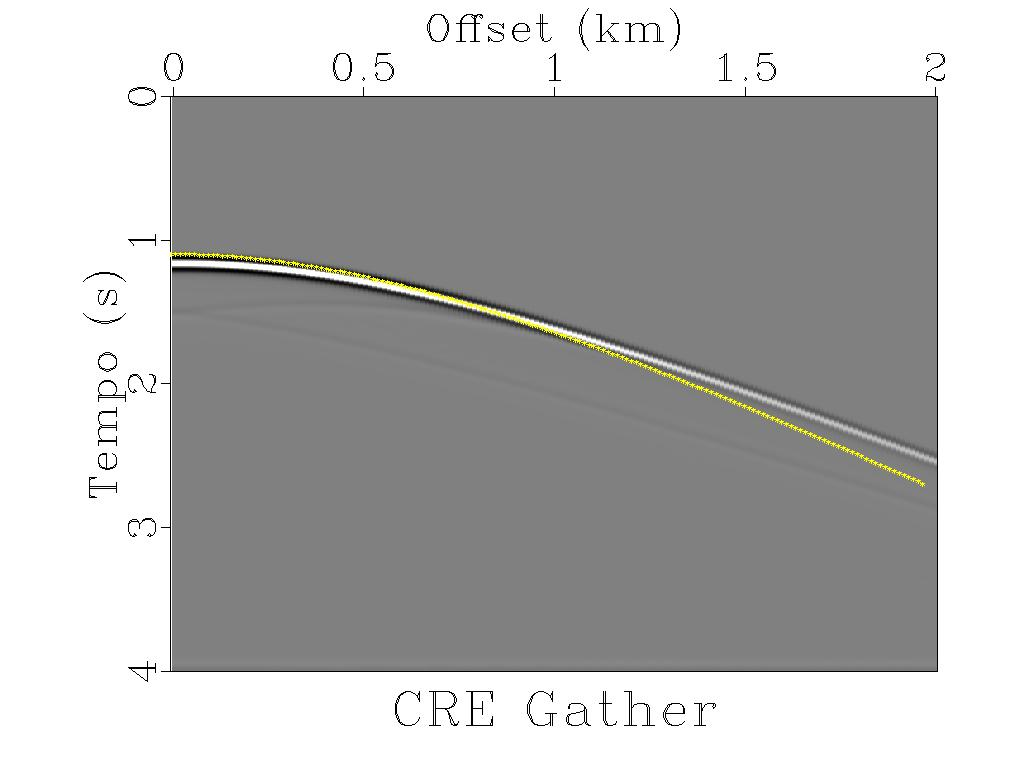
\includegraphics[scale=0.3]{images/interpolacao5.jpeg}
\vspace{-0.3cm}
\end{center}
\begin{center}
 Fonte: Do Autor.
\end{center}
\label{fig:6.1}
\end{figure}

\begin{figure}
\caption{Seção CRE para o PMC $m0=4Km$ e $t0=1.3s$.
Pontos em amarelo representa a curva de tempo de trânsito ERC sobre a qual
será realizado o empilhamento ERC.
O eixo horizontal é a coordenada do afastamento $h$ e o eixo vertical o tempo
$t$.}
\begin{center}
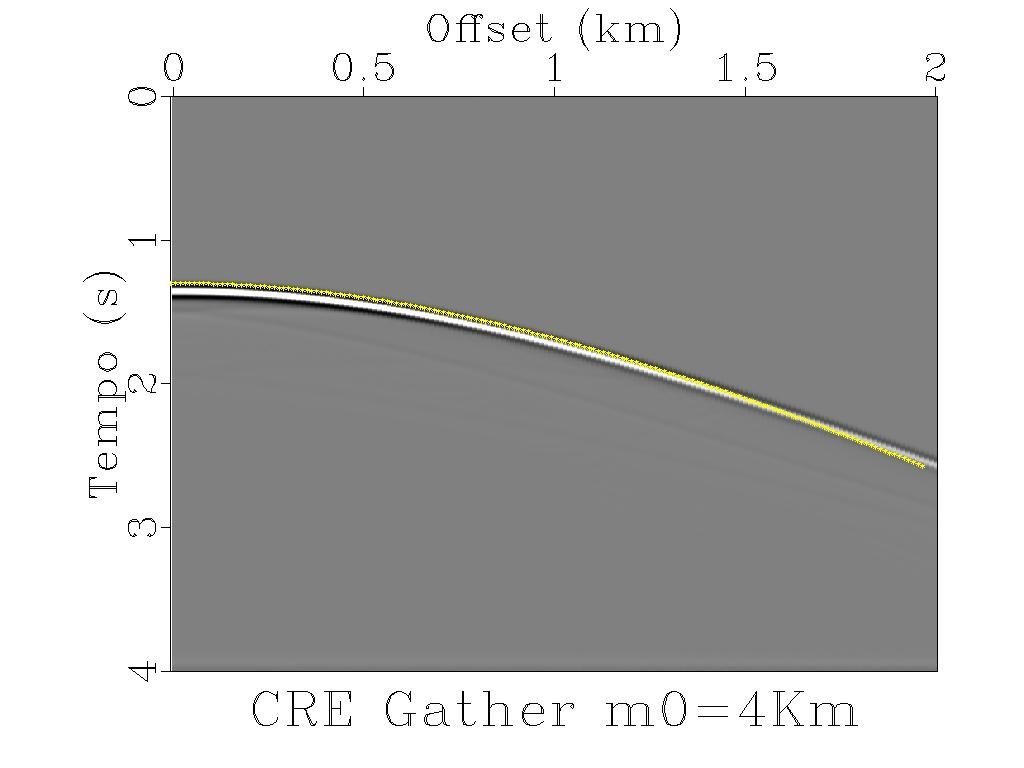
\includegraphics[scale=0.3]{images/interpolacao4.jpeg}
\vspace{-0.3cm}
\end{center}
\begin{center}
 Fonte: Do Autor.
\end{center}
\label{fig:6.2}
\end{figure}

\begin{figure}
\caption{Seção CRE para o PMC $m0=4Km$ e $t0=1.1s$.
Pontos em amarelo representa a curva de tempo de trânsito ERC sobre a qual
será realizado o empilhamento ERC.
O eixo horizontal é a coordenada do afastamento $h$ e o eixo vertical o tempo
$t$. A escolha de $t0=1.1$ não produziu o melhor ajuste da curva ERC aos dados modelados.}
\begin{center}
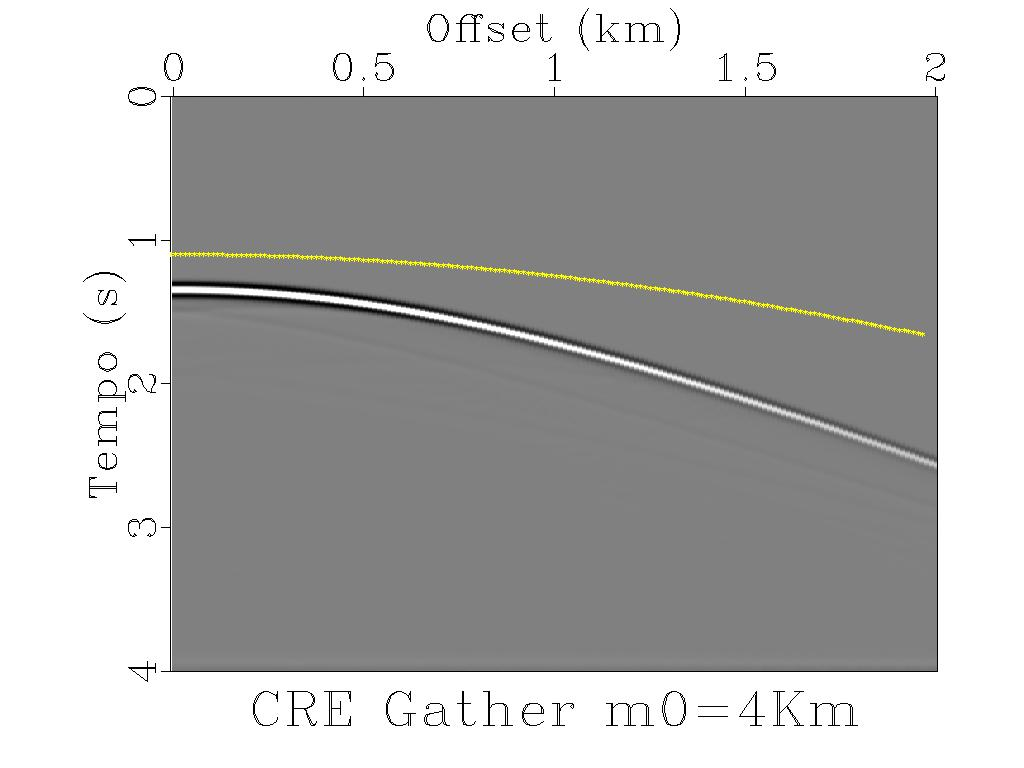
\includegraphics[scale=0.3]{images/interpolacaoErro.jpeg}
\vspace{-0.3cm}
\end{center}
\begin{center}
 Fonte: Do Autor.
\end{center}
\label{fig:6.3}
\end{figure}
